\chapter{Reinforcement Learning Approach}

\section{Brief Description}
Reinforcement learning works by learning to map the 
state of the system to the choice of available actions based on long-term reward 
(or penalty). In this report we will discuss review in brief the prior work \cite{ARTICLE:1} and then discuss the work that will be done as part of the project.  The key difference in both the
the approaches is:
\begin{itemize}
\item In the prior approach, we find state space with respect to train and it is the train that is making the 
decision (So we have the environment where each train is acting as the agent i.e. multiagent environment) 
\item In the proposed work, we have the central controller as the single agent and it is that
agent that is scheduling the trains.
\end{itemize}

\section {Prior Work}
\subsection{State Representation (Local state space)}

Here, we compute the state space as a function of \textbf{local neighborhood} of each
train.
A state vector is computed for each train every time a
decision about its next move is to be computed. Relative to
the direction of motion, we define resources as being behind
(in the direction opposite to the direction of motion) or in
front (in the direction of motion) of the train. A user-defined
finite number of resources $ l_b $ behind each train and $ l_f $ in
front of each train are used for defining the state vector. These
are referred to as local resources. Including a few resources
behind the train in the state definition ensures that overtaking
opportunities for fast-moving trains are not missed. The total
number of local resources is ($ l_b + 1 + l_f $). 
\vspace{0.2cm}
\begin{figure}[h]
    \centering
    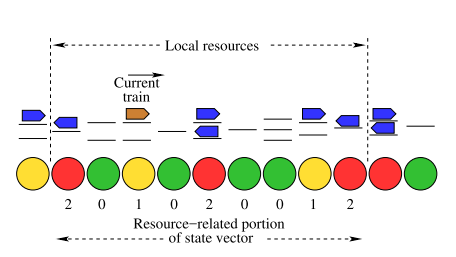
\includegraphics[width=0.8\textwidth]{report2}
    \caption{ Mapping train location and direction of movement to resource
    status, relative to the ‘current train’ \cite{ARTICLE:1}.  }
    \label{image-myimage}
\end{figure}


The entry in the state vector corresponding to each local
resource takes one of R integer values $ \{0, 1, 2,..., R-1\} $,
referred to as the status $S_r$ of resource $r$. Higher values
indicate higher congestion within the resource, and are driven
by the number of occupied tracks.
Let us define the number
of tracks in resource r to be equal to $N_r$, out of which $T_{r,c}$
tracks contain trains converging with (heading towards) the
current train, while $T_{r,d}$ tracks contain trains diverging from
(heading away from) the current train. Since at most one train
can occupy a given track, we note that $T_{r,c} + T_{r,d} < N_r$. The
mapping from track occupancy to resource status is,

$$ S_r = R - 1 - min(R - 1, \left \lceil{N_r - w_c T_{r,c} - w_d T_{r,d} }\right \rceil ).$$

Here, $0 \leq w_c$, $w_d \leq 1$ are weights that can de-emphasise
the effect of converging and diverging trains on the perceived
status of a resource.
\vspace{0.2cm}
We have one more entry in the state space for the priority of trains. If we assume that the model accommodates
up to $P$ priority levels, the size of the state space is equal to
\textbf { $ P \cdot R^{l_b+1+l_f} $}. Note that this value does not depend on the
scale of the problem instance, in terms of the number of trains,
the lengths of their journeys, and the number of resources.

\subsection {Action and Policy Definition}

In this approach, state space is computed for each train locally. 
The choice of actions in any given state is binary, with
0 representing a decision to move the current train to the next
resource on its journey, and 1 representing a decision to halt
in the current resource for a predefined time period (1 minute
in this paper). If the train is halted, the decision-making
procedure is repeated after the time period elapses.
 The policy that can be used to take the action is $ \epsilon$-greedy with the 
 value of $ \epsilon$-decresing over the training. It comprise of three steps 
 \begin{itemize}
\item Select the train on which to take the action.
\item Compute the state space for the train. 
\item Choose the action depending on the $\epsilon$-greedy policy. 
 \end{itemize}

\section{Proposed Approach}
\subsection {State Space Representation}
We are planning to use the whole network along with the positions of each train to take
as the state space. The key idea is to let the RL algorithm find which part of the state 
space is important to make decision. In the prior approach, we are kind of tuning how far the train can see and it's
action depends only on local neighborhood but in our work we are going to include everything in the state space.
Since, including everything can blow the size of the state space really quickly, so to tackle with this 
problem we can use function approximation methods (Deep Q-Learning) to learn the state space and then 
work on it.
\subsection{Action And Policy Definition}

In our proposed approach, we take the whole network topology and the position of the trains as the 
state space. So we have the central controller and that central controller will take the action for each train depending on 
state space that takes everything into account. 
At a particular time during the simulation, let's say we have n number of trains waiting for the 
action (ready to move or stop), then the controller have the action space of $2^n$ and it has to 
make decision for each of the trains (although in some order, as we are running the simulator and taking action 
for one train at a time).Size of the action space depends on the number of trains waiting for the 
action to be taken. Here again we can use the $\epsilon$-greedy policy for exploration in the initial phase
and then further exploitation.

\section {Objective Function}
A number of objective functions have been used in the
railway scheduling context, in order to achieve goals such
as delay reduction, passenger convenience, and timetable
robustness. One of the commonly used measures of
schedule quality is priority-weighted delay. A delay is
defined to be the non-negative difference between the time
of an event as computed by the algorithm, and the desired
time as specified by the timetable. The priority-weighted
average delay is the mean over all trains and all stations
of individual delays divided by train priorities. This quantity
is used as the objective function, but the algorithm can
accommodate other measures equally easily (for example,
a non-linear function of delays in order to increase fairness
of delay distribution).
$$ J = \frac{1}{N_{r,t}} \sum_{r,t} \frac{\delta_{r,t}}{P_t} $$
where $\delta_{r,t}$ is the delay for train t on departure from resource r,
$p_t$ is the priority of train t, and $N_{r,t}$ is the total number of
departures in the schedule. Note that this expression includes
all events for all trains, for their entire journey.

Prior work uses priority weighted delay as the objective function. In our proposed 
approach as well, we can shape the reward functions as to use the same
objective function.
